% Current version: v2.2b
% Author: Wenhao Wu, Kun Wang, Zhi Ding, Chengshan Xiao
% Email: {wnhwu,kunwang,zding}@ucdavis.edu, xiaoc@mst.edu}
% Date: 11/02/2013
% Update:
%   -
% Substitute version: v2.2
% Author: Wenhao Wu, Kun Wang, Zhi Ding, Chengshan Xiao
% Email: {wnhwu,kunwang,zding}@ucdavis.edu, xiaoc@mst.edu}
% Date: 11/02/2013
% Update:
%   - Revised by Prof. Xiao
%   - Multiple reference style corrected ([1][2] -> [1, 2])
%   - Spacing and comma
%   - Add 1 and delete 1 reference.
%   - Reference author first and middle name initialized
%   - Reference abbreviation capitalized
%
% Substitute version: v2.1
% Author: Wenhao Wu, Kun Wang, Zhi Ding, Chengshan Xiao
% Email: {wnhwu,kunwang,zding}@ucdavis.edu, xiaoc@mst.edu}
% Date: 11/01/2013
% Update:
%   - Difference between v2.0 and v1.2 noted
%   - Minor inconsistence removed
%
% Substitute version: v2.0
% Author: Wenhao Wu, Kun Wang, Zhi Ding, Chengshan Xiao
% Email: {wnhwu,kunwang,zding}@ucdavis.edu, xiaoc@mst.edu}
% Date: 10/31/2013
% Update:
%   - Revised by Prof. Ding
%
% Substitute version: v1.2
% Author: Wenhao Wu, Kun Wang, Zhi Ding, Chengshan Xiao
% Email: {wnhwu,kunwang,zding}@ucdavis.edu, xiaoc@mst.edu}
% Date: 10/30/2013
% Update:
%   - BDAGDP algorithm description modified
%   - More major parameters specifications in simulation description
%   - GP1-SGDP figure completed.
%
% Substitute version: v1.1
% Author: Wenhao Wu, Kun Wang, Zhi Ding, Chengshan Xiao
% Email: {wnhwu,kunwang,zding}@ucdavis.edu, xiaoc@mst.edu}
% Date: 10/29/2013
% Update:
%   - Equation (7)(8) compressed
%   - Short last line eliminated
%   - Figure line color for QPSK turned from green to purple
%
% Substitute version: v1.0
% Author: Wenhao Wu, Kun Wang, Zhi Ding, Chengshan Xiao
% Email: {wnhwu,kunwang,zding}@ucdavis.edu, xiaoc@mst.edu}
% Date: 10/21/2013
%
% Codename: New Columbia
% --------------------------------------------------------------------------
% Template for ICASSP-2014 paper; to be used with:
%          spconf.sty  - ICASSP/ICIP LaTeX style file, and
%          IEEEbib.bst - IEEE bibliography style file.
% --------------------------------------------------------------------------

\documentclass{article}
\usepackage{spconf,amsmath,graphicx,epstopdf,amsfonts,mathtools,bm,float,afterpage}

% Example definitions.
% --------------------
\def\x{{\mathbf x}}
\def\L{{\cal L}}

\hyphenation{BC}
\hyphenation{BD}
\hyphenation{term}
\hyphenation{BS}
\hyphenation{MS}
\hyphenation{MIMO}
% Title.
% ------
\title{Cooperative Multi-Cell MIMO Downlink Precoding for Finite-Alphabet Inputs} % Mod_Ding: Title shortened

%
% Single address.
% ---------------
\name{Wenhao Wu$^\star$ \qquad Kun Wang$^\star$ \qquad Zhi Ding$^\star$ \qquad Chengshan Xiao$^\dagger$\thanks{This material is based on
 works supported by the National Science Foundation Grants CNS-1147930, ECCS-1307820 and CIF-1321143.}}
\address{$ $\\
\vspace*{-14mm}\\
$^\star$Department of Electrical and Computer Engineering,\\
 University of California, Davis, CA 95616 \\
$^\dagger$Department of Electrical and Computer Engineering, \\
Missouri University of Science and Technology, Rolla, MO 65409\\
\texttt{$^\star$\{wnhwu,kunwang,zding\}@ucdavis.edu, $^\dagger$xiaoc@mst.edu} \\
\vspace*{-12mm}
 }


\begin{document}
%\ninept
%
\maketitle
%
\begin{abstract}
    % (what we do)
    This work studies the design of linear precoders for cooperative multi-cell MIMO downlink
    systems with finite alphabet inputs.
    % (how they do)
    Traditionally, multi-cell MIMO downlink precoder designs rely on Gaussian input assumption, which may lead to
    performance loss when the true inputs admit discrete non-Gaussian symbols. % Mod_Ding: revised
    % (how we do)
    In this work, we present optimized precoders by maximizing weighted sum rate
    (of finite-alphabet-input) under a set of per-base station power constraints. Specifically,
    we propose a simple gradient algorithm for general multi-cell MIMO downlink channel and a block diagonalization gradient
   algorithm while
    supporting interference cancellation. % Mod_Ding: BDAGDP description reversed
    % (main results)
    %Simulation results demonstrate significant gain over some Gaussian input-based precoding schemes.
\end{abstract}

\begin{keywords}
    Multi-cell downlink , linear precoding, finite-alphabet input, gradient descent, dual decomposition.
\end{keywords} % Mod_Ding: multi-cell downlink (channel)
\vspace*{-3mm}

\section{Introduction}
\label{sec:intro}
\vspace*{-2mm}

% Why are we interested in precoder optimization to maximize WSR in multi-cell MIMO downlink channel
Cooperative transmission in multi-cell MIMO downlink channel (MC-MIMO-DLC) has been a topic
that attracted growing interest in recent years,
as a promising technology for cellular interference management. Among various approaches,
cooperative precoding has shown substantial rate improvement when given channel state information (CSI) and
when data streams are available to all base stations (BSs) \cite{gesbert2010multi}.
An MC-MIMO-DLC resembles MIMO broadcasting channel (BC) except for the stricter
per-BS (or per-antenna) power constraints
(rather than the sum-power constraint). %\cite{biglieri2007mimo}.
Although the uplink-downlink duality and capacity-reaching dirty paper coding (DPC) scheme
can be generalized \cite{yu2007transmitter, huh2009mimo}, their implementation
difficulty has made suboptimal precoder design such as linear precoders more favorable.

% Unlike existing approach based on Gaussian, our approach is based on finite-alphabet inputs
While existing linear precoder design approaches for MC-MIMO-DLC are mostly based on Gaussian input assumption,
practical communication systems have input signals from finite-alphabet constellation. This
difference leads to considerable gap between the actual rate and the capacity.  Such mismatch
can often degrade the performance of Gaussian input based methods.
Noting this key discrepancy and mismatch, our linear precoder designs for MC-MIMO-DLC shall specifically target finite-alphabet
inputs.

% Other methods in multicell MIMO downlink; finite-alphabet inputs assumption for other models - what is missing
There exist several linear precoder design algorithms for maximizing weighted sum rate (WSR) in MC-MIMO-DLC.
Due to the non-convexity of the problem formulation, most of them rely on numerical alternating  methods,
including mean square error (MSE) receiver/weighting matrix update - precoder optimization \cite{christensen2008weighted, fritzsche2013robust},
and interference/leakage update - precoder optimization \cite{wang2012coordinated}. When block diagonalization (BD) constraint can be enforced,
the MC-MIMO-DLC becomes simpler and the WSR maximization problem with per-BS power constraints becomes, convex.
A dual-decomposition based, cooperative, multi-cell BD precoder design method is proposed
in \cite{zhang2010cooperative} and  two other suboptimal solutions are provided in \cite{zhang2009networked}.
As a special case, beamforming of MC-MIMO-DLC can be found in \cite{venturino2010coordinated, zhang2010cooperativeinter}.

Although the aforementioned studies are all based on Gaussian input assumption, linear precoder
optimization for finite alphabet inputs has been investigated for several scenarios including single user MIMO \cite{perez2010mimo, xiao2011globally},
MIMO BC \cite{wu2012linear}, MIMO multiple access channels (MAC) \cite{wang2011linear}, MIMO relay channels \cite{liang2012linear, zeng2012linearrelay},
MIMO hybrid-ARQ (HARQ) \cite{liang2011sequential}, as well as MIMO wiretap channels \cite{wu2012linearMIMOME}.
Each case demonstrates performance gain over the laissez faire use of their Gaussian based precoder design counterpart.

% My contribution (emphasize difference from related works)
To the best of our knowledge, there has been scant research on precoder design for MC-MIMO-DLC under finite-alphabet inputs.
In this work, we examine the linear finite-alphabet precoder design problem in MC-MIMO-DLC under per-BS power constraint.
We first derive a simple gradient-descent precoder optimization algorithm. To avoid the time-consuming Monte-Carlo numerical evaluation,
we generalize the rate approximation and its gradient in \cite{zeng2012low} to MIMO-BC model \cite{wu2012linear} while incorporating the per-BS constraint.
Next, we include the BD restriction to our precoder design scheme and subsequently decompose the WSR objective into single user rate objectives.
We enable a nontrivial extension of the alternating optimization algorithm in \cite{xiao2011globally}. This is achieved by applying the dual-decomposition technique \cite{zhang2010cooperative, palomar2006tutorial} to the newly formulated convex power allocation subproblems under per-BS power constraints.
Our numerical test results show that both our proposed design algorithms outperforms the Gaussian based designs,
particularly in the medium SNR regime.
% Mod_Ding: More concise, vspace specified
\vspace*{-3mm}

\section{System Model and Problem Formulation}
\label{sec:mode}
\vspace*{-2mm}


% multi-cell MIMO downlink channel
Consider a cellular network consisting of $A$ cells, each having a BS with $N_t$ Tx antennas.
The $a$-th cell has $K_a$ mobile stations (MSs) each equipped with $N_r$ Rx antennas.
The total number of MSs is $K = \sum_{a=1}^AK_a$ and the total number of TX antennas equals $N=AN_t$.
The received signal at the $k$-th MS is given by
\begin{equation}
    \label{eq:channel}
    \mathbf{y}_k = \mathbf{H}_k\mathbf{x}_k+\sum_{i\not=k}\mathbf{H}_k\mathbf{x}_i+\mathbf{z}_k,\;k=1,\ldots,K
\end{equation}
in which $\mathbf{x}_k\in\mathbb{C}^{N_t\times1}$ is the transmitted signal vector intended for the $k$-th MS.
$\mathbf{H}_k\in\mathbb{C}^{N_r\times N}$ is the normalized channel matrix from the virtual BS formed by the set of
cell BSs to the $k$-th MS with $\mbox{tr}\left(\mathbf{H}_k\mathbf{H}_k^H\right)=N_r$. $\mathbf{z}_k\sim\mathcal{CN}(\mathbf{0},\sigma^2\mathbf{I})$ is receiver
noise. We assume a full cooperative scheme where the channel state information (CSI) is perfectly known to all BSs and MSs involved.

The linear precoding is represented as
\begin{equation}
    \label{eq:precoder}
    \mathbf{x}_k = \mathbf{P}_k\mathbf{s}_k,\;k=1,\ldots,K
\end{equation}
where $\mathbf{P}_k\in\mathbb{C}^{N\times N_r}$ denotes the precoder and $\mathbf{s}_k\in\mathbb{C}^{N_r\times1}$
denotes the finite-alphabet data vector for the $k$-th MS. Elements in $\mathbf{s}_k$ is independent and uniformly
distributed from a
constellation of size $M$, with zero mean and unit variance.

% WSR Maximization under per-BS Power Constraints
Throughout this paper, we strive to maximize the weighted sum rate as a function of the precoders
\begin{equation}
    \label{eq:WSR}
    R(\{\mathbf{P}_k\}) = \sum_{k=1}^K\mu_kR_k(\{\mathbf{P}_k\})
\end{equation}
where the $k$-th MS achievable rate  $R_k(\{\mathbf{P}_k\})$   is the same as its counterpart in MIMO-BC given by \emph{Proposition 1} in \cite{wu2012linear}.
Let $N_t$ be the normalized maximum transmit power of each BS. The per-BS power constraints are given by
\begin{equation}
    \label{eq:perBSpwrConstr}
    \sum_{k=1}^K\|\mathbf{B}_a\mathbf{P}_k\|_F^2 = \sum_{k=1}^K\mbox{tr}\left(\mathbf{B}_a\mathbf{P}_k\mathbf{P}_k^H\right) \leq N_t,\;a=1,\ldots,A
\end{equation}
with Frobenius norm $\|\cdot\|_F$ while $\mathbf{B}_a$ is defined in \cite{zhang2010cooperative} as
\begin{equation}
    \label{eq:Ba}
    \mathbf{B}_a\coloneqq\mbox{Diag}(\underbrace{0,\ldots,0}_{(a-1)N_t},\underbrace{1,\ldots,1}_{N_t},\underbrace{0,\ldots,0}_{(A-a)N_t}).
\end{equation}

% Challenges beyond Existing Works
The challenges from this new formulation beyond existing works are twofold. First, this constrained optimization
problem is non-convex, which compels the search for suboptimal solutions. Second, evaluating the
finite-alphabet rate $R_k(\{\mathbf{P}_k\})$ in Eq. (\ref{eq:WSR}) requires time-consuming Monte-Carlo
statistical sampling for non-trivial model settings. In the following section, we will address these
two challenges in the development of our algorithms.  % Mod_Ding: More concised


\vspace*{-4mm}

\section{Precoder Design}
\label{sec:pd}
\vspace*{-3mm}

    \subsection{Simple Gradient-Descent Precoder (S-GDP)}
    \label{ssec:SGDP}
    \vspace*{-2mm}

    Gradient descent method is a common way for finding local optima \cite{boyd2004convex}.
Our obstacle lies in the need to repeatedly evaluate the rate (for finite-alphabet inputs) and its gradient using
    computationally costly Monte-Carlo. This is particularly costly for MC-MIMO-DLC as the interferences are also finite-alphabetical.
    To tackle this problem, we generalize the approximation for non-interference channel in \cite{zeng2012low} to the interference channel in our problem.

    % Mod_Ding: intro and description splitted, more concise
    Denote constellation vector index set $\mathbb{I}=\{1,\ldots,M\}$ and its $K$-ary and $(K-1)$-ary Cartesian products as $\mathbb{A}=\{(p_1,\ldots,p_K)|p_i\in\mathbb{I}\}$ and $\mathbb{A}_k=\{(p_1,\ldots,p_K)|p_i\in\mathbb{I},i\not=k\}$, respectively. Then the approximation to $R_k(\{\mathbf{P}_k\})$ is given by
    \begin{align}
        \hat{R}_k(\{\mathbf{P}_k\}) & = \log_2M + \frac{1}{M^{K-1}} \sum_{\mathbf{m}_k\in \mathbb{A}_k}\log_2\sum_{\mathbf{n}_k\in \mathbb{A}_k}u_{\mathbf{m}_k\mathbf{n}_k}
        \nonumber\\
                                    & - \frac{1}{M^K}\sum_{\mathbf{m}\in \mathbb{A}}\log_2\sum_{\mathbf{n}\in \mathbb{A}}v_{\mathbf{m}\mathbf{n}}
        \label{eq:ARSGDP}
    \end{align}
    in which
$u_{\mathbf{m}_k\mathbf{n}_k}=\exp(-\mathbf{c}_{\mathbf{m}_k\mathbf{n}_k}^H\mathbf{c}_{\mathbf{m}_k\mathbf{n}_k}/2\sigma^2)$
and
$
 v_{\mathbf{m}\mathbf{n}}=\exp(-\mathbf{d}_{\mathbf{m}\mathbf{n}}^H\mathbf{d}_{\mathbf{m}\mathbf{n}}/2\sigma^2),
$    where $\mathbf{c}_{\mathbf{m}_k\mathbf{n}_k}=\mathbf{H}_k\sum_{j\not=k}\mathbf{P}_j\mathbf{e}_{m_j,n_j}$ and $\mathbf{d}_{\mathbf{m}\mathbf{n}}=\mathbf{H}_k\sum\mathbf{P}_j\mathbf{e}_{m_jn_j}$.
    Here $m_j,\,n_j$ are the entries of index vectors $\mathbf{m}_k/\mathbf{m}$ and ${\mathbf{n}_k/\mathbf{n}}$, and $\mathbf{e}_{m_jn_j} = \mathbf{s}^{(m_j)}-\mathbf{s}^{(n_j)}$ denotes the difference between the $m_j$-th and $n_j$-th constellation vectors.

    The gradient of $\hat{R}_k(\{\mathbf{P}_k\})$ with respect to (w.r.t.)  precoder $\mathbf{P}_i$, according to \cite{hjorungnes2011complex}, is given by
    \begin{equation}
        \label{eq:gradARSGDP1}
        \begin{aligned}
            & \nabla_{\mathbf{P}_i}\hat{R}_k|_{i\not=k} = -\frac{\mathbf{H}_k^H\mathbf{H}_k}{2\ln2\sigma^2}\\
            & \left(\sum_{\mathbf{m}_k\in \mathbb{A}_k}\frac{\sum_{\mathbf{n}_k\in \mathbb{A}_k}u_{\mathbf{m}_k\mathbf{n}_k}\left(\sum_{j\not=k}\mathbf{P}_j\mathbf{e}_{m_jn_j}\right)\mathbf{e}_{m_in_i}^H}{M^{K-1}\sum_{\mathbf{n}_k\in \mathbb{A}_k}u_{\mathbf{m}_k\mathbf{n}_k}}\right. \\
            & \left. - \sum_{\mathbf{m}\in \mathbb{A}} \frac{\sum_{\mathbf{n}\in \mathbb{A}}v_{\mathbf{m}\mathbf{n}}\left(\sum\mathbf{P}_j\mathbf{e}_{m_jn_j}\right)\mathbf{e}_{m_in_i}^H}{M^K\sum_{\mathbf{n}\in \mathbb{A}}v_{\mathbf{m}\mathbf{n}}}\right)
        \end{aligned}
    \end{equation}
    \begin{equation}
        \label{eq:gradARSGDP2}
        \begin{aligned}
            \nabla_{\mathbf{P}_k}\hat{R}_k & = -\frac{\mathbf{H}_k^H\mathbf{H}_k}{2\ln2\sigma^2}\sum_{\mathbf{m}\in \mathbb{A}}\frac{\sum_{\mathbf{n}\in \mathbb{A}}v_{\mathbf{m}\mathbf{n}}\left(\sum\mathbf{P}_j\mathbf{e}_{m_jn_j}\right)\mathbf{e}_{m_kn_k}^H}{M^K\sum_{\mathbf{n}\in \mathbb{A}}v_{\mathbf{m}\mathbf{n}}}. \\
        \end{aligned}
    \end{equation}
    To enforce the per-BS power constraints during gradient descent, we project the updated precoders to a feasible solution
    in each iteration. \cite{zhang2004cochannel} discussed several projection methods.
    Here we use a straightforward projection $\mbox{Proj}(\mathbf{P}_k)=\mathbf{TP}_k$ where $\mathbf{T}$ is a $N$-by-$N$ block-diagonal matrix
    with its $a$-th $N_t$-by-$N_t$ block-diagonal element as:
    \begin{equation}
        \label{eq:Proj}
           \mathbf{T}_a = \left\{
                             \begin{array}{ll}
                                   \mathbf{I}_{N_{t}} & \mbox{if } \sum_{k=1}^K\|\mathbf{B}_a\mathbf{P}_k\|_F^2 \leq N_t; \\
                                   \frac{\sqrt{P}\mathbf{I}_{N_{BS}}}{\sum_{k=1}^K\|\mathbf{B}_a\mathbf{P}_k\|_F^2} & \mbox{otherwise.}
                             \end{array}
                          \right.
    \end{equation}

    Now we are ready to summarize the steps of our Simple Gradient-Descent Precoder (S-GDP) optimization algorithm: % Mod_Ding: precoder renamed
    \begin{enumerate}\itemsep0pt\parskip0pt\parsep0pt
        \item[S1] Select a feasible set of initial precoders $\{\mathbf{P}_k\}$.
        \item[S2] Evaluate the approximated weighted sum rate (AWSR) $\hat{R}(\{\mathbf{P}_k\}) = \sum_{k=1}^K\mu_k\hat{R}_k(\{\mathbf{P}_k\})$ and its gradients $\nabla_{\mathbf{P}_i}\hat{R}(\{\mathbf{P}_k\}) = \sum_{k=1}^K\mu_k\nabla_{\mathbf{P}_i}\hat{R}_k(\{\mathbf{P}_k\})$ for $i=1,\ldots,K$. Determine the step size $t$ with backtracking line search method \cite{boyd2004convex}.
        \item[S3] For $k=1,\ldots,K$, evaluate $\mathbf{P}_k^* = \mathbf{P}_k + t\nabla_{\mathbf{P}_k}\hat{R}(\{\mathbf{P}_k\})$. Then get the updated precoders by $\mathbf{P}_k \leftarrow \mathbf{TP}_k^*$.
        \item[S4] Return to S2 until convergence.
    \end{enumerate}

    \vspace*{-3mm}

    \subsection{Block Diagonalization - Alternating Gradient-Descent Precoder (B-GDP)}  % Mod_Ding: precoder renamed
    \label{ssec:BDAGDP}
    \vspace*{-2mm}

    Although the S-GDP algorithm is straightforward, the interference term makes $\hat{R}(\{\mathbf{P}_k\})$ highly non-convex.
    Thus, we need good initial precoders to achieve good performance.
    Each MS also needs to decode the finite-alphabet interference for rate benefit.
    Moreover, computational complexity required for evaluating $\hat{R}_k$ and $\nabla_{\mathbf{P}_k}\hat{R}_k$
    grows rapidly following $\mathcal{O}(K ^ 2NN_r(M^ {2K} + N))$  w.r.t $K$. However, when $N \geq KN_r$,
    it is possible to focus on block-diagonalization (BD) precoding scheme that is substantially simpler and
    performs well in high SNR regime.  BD achieves some convex property and reduces computational complexity.

    Denote $\mathbf{G}_k=[\mathbf{H}_1^T,\ldots,\mathbf{H}_{k-1}^T,\mathbf{H}_{k+1}^T, \ldots , \mathbf{H}_{K}^T]^T$
    whose null space $\bar{\mathbf{V}}_{\mathbf{G}_k}$ can be derived from the singular vector decomposition (SVD) as $\mathbf{G}_k = \mathbf{U}_{\mathbf{G}_k}
    \bm{\Sigma}_{\mathbf{G}_k}[\mathbf{V}_{\mathbf{G}_k},\bar{\mathbf{V}}_{\mathbf{G}_k}]^H$. By restricting $\mathbf{P}_k = \bar{\mathbf{V}}_{\mathbf{G}_k}\bar{\mathbf{P}}_k$,
the interference-free channel for the $k$-th MS is $\bar{\mathbf{H}}_k = \mathbf{H}_k\bar{\mathbf{V}}_{\mathbf{G}_k}$.
Denote the SVD of $\bar{\mathbf{P}}_k$ as $\bar{\mathbf{P}}_k = \mathbf{U}_{\bar{\mathbf{P}}_k}\mathbf{\Sigma}_{\bar{\mathbf{P}}_k}\mathbf{V}_{\bar{\mathbf{P}}_k}^H$.
Although \emph{Proposition 2} in \cite{xiao2011globally} is no longer valid due to per-BS power constraints, we can still get the following equivalent channel if
we align $\mathbf{U}_{\bar{\mathbf{P}}_k}$ to the right singular vectors of $\bar{\mathbf{H}}_k$, as if the inputs were Gaussian or we were considering a point-to-point MIMO system with finite alphabet inputs \cite{payaro2009optimal}:
    \begin{equation}
        \label{eq:channelBDEQ}
        \bar{\mathbf{y}}_k=\mathbf{\Sigma}_{\bar{\mathbf{H}}_k}\mathbf{\Sigma}_{\bar{\mathbf{P}}_k}\mathbf{V}_{\bar{\mathbf{P}}_k}^H\mathbf{s}_k+\bar{\mathbf{z}}_k.
    \end{equation}

    The approximated rate for the $k$-th MS is \cite{zeng2012low}
    \begin{equation}
        \label{eq:ARBDAGDP}
        \bar{R}_k(\mathbf{\Sigma}_{\bar{\mathbf{P}}_k}^2,\mathbf{V}_{\bar{\mathbf{P}}_k}) = \log_2M - \frac{1}{M}\sum_{m=1}^{M}\log_2\sum_{n=1}^Mw_{mn}
    \end{equation}
    where $w_{mn} = \exp(\mathbf{e}_{mn}^H\mathbf{W}_k\mathbf{e}_{mn}/2\sigma^2)$, $\mathbf{e}_{mn}=\mathbf{s}^{(m)}-\mathbf{s}^{(n)}$ and $\mathbf{W}_k=\mathbf{V}_{\bar{\mathbf{P}}_k}\mathbf{\Sigma}_{\bar{\mathbf{P}}_k}^2\mathbf{\Sigma}_{\bar{\mathbf{H}}_k}^2\mathbf{V}_{\bar{\mathbf{P}}_k}^H$. Its gradient w.r.t $\mathbf{W}_k$ is
    \begin{equation}
        \label{eq:gradWARBDAGDP}
        \nabla_{\mathbf{W}_k}\bar{R}_k=\sum_{m=1}^M\frac{\sum_{n=1}^Mw_{mn}(\mathbf{e}_{mn}\mathbf{e}_{mn}^H)}{2\ln2\sigma^2M\sum_{n=1}^Mw_{mn}}.
 \end{equation}

    Similar to \cite{xiao2011globally}, we attempt to maximize the AWSR by alternatingly solving
    \begin{align}
        \label{eq:optVPk}
     &   \max \bar{R}_k(\mathbf{V}_{\bar{\mathbf{P}}_k}|\mathbf{\Sigma}_{\bar{\mathbf{P}}_k}^2), k=1,\ldots,K;
\\
      & \max \sum\nolimits_{k=1}^K\mu_k\bar{R}_k(\mathbf{\Sigma}_{\bar{\mathbf{P}}_k}^2|\mathbf{V}_{\bar{\mathbf{P}}_k}),                     \label{eq:optSigmaP}\\
            \mbox{s.t. } &  % Mod_Ding: qquad used
            \sum\nolimits_{k=1}^K\mbox{tr}(\mathbf{B}_a\bar{\mathbf{V}}_{\mathbf{G}_k}\mathbf{V}_{\bar{\mathbf{H}}_k}\mathbf{\Sigma}_{\bar{\mathbf{P}}_k}^2\mathbf{V}_{\bar{\mathbf{H}}_k}^H\bar{\mathbf{V}}_{\mathbf{G}_k}^H)\leq N_t.\nonumber
\end{align}

    Problem (\ref{eq:optVPk}) can be solved with a Stiefel manifold based method \cite{zeng2012linearrelay} in which the line-search direction is
    \begin{equation}
        \label{eq:deltaVBDAGDP}
        \Delta\mathbf{V}_{\bar{\mathbf{P}}_k} = \nabla_{\mathbf{V}_{\bar{\mathbf{P}}_k}}\bar{R}_k - \mathbf{V}_{\bar{\mathbf{P}}_k}(\nabla_{\mathbf{V}_{\bar{\mathbf{P}}_k}}\bar{R}_k)^H\mathbf{V}_{\bar{\mathbf{P}}_k},
    \end{equation}
    \begin{equation}
        \label{eq:gradVBDAGDP}
        \nabla_{\mathbf{V}_{\bar{\mathbf{P}}_k}}\bar{R}_k = (\nabla_{\mathbf{W}_k} \bar{R}_k)^H \mathbf{V}_{\bar{\mathbf{P}}_k}\Sigma_{\bar{\mathbf{P}}_k}^2\Sigma_{\bar{\mathbf{H}}_k}^2.
    \end{equation}

    The convex problem (\ref{eq:optSigmaP}) can be solved by dual decomposition \cite{zhang2010cooperative, palomar2006tutorial}. Denote $\bm{\gamma}=(\gamma_1,\ldots,\gamma_A)^T\succeq \mathbf{0}$ as the dual variables. We alternatingly solve the $K$ individual subproblems $\max f_k(\mathbf{\Sigma}_{\bar{\mathbf{P}}_k}^2|\bm{\gamma})$, $k=1,\ldots,K$, where
    \begin{equation}
        \label{eq:fk}
        \begin{aligned}
            f_k(\mathbf{\Sigma}_{\bar{\mathbf{P}}_k}^2, \bm{\gamma}) & = \mu_k\bar{R}_k(\mathbf{\Sigma}_{\bar{\mathbf{P}}_k}^2|\mathbf{V}_{\bar{\mathbf{P}}_k}) \\
            & - \mbox{tr}(\mathbf{B}_{\bm{\gamma}}\bar{\mathbf{V}}_{\mathbf{G}_k}\mathbf{V}_{\bar{\mathbf{H}}_k}\mathbf{\Sigma}_{\bar{\mathbf{P}}_k}^2\mathbf{V}_{\bar{\mathbf{H}}_k}^H\bar{\mathbf{V}}_{\mathbf{G}_k}^H)
        \end{aligned}
    \end{equation}
    and $\mathbf{B}_{\bm{\gamma}} = \sum_{a=1}^A\gamma_a\mathbf{B}_a$ with the barrier function - gradient descent - backtracking line search method \cite{zeng2012linearrelay, boyd2004convex} and solve the primal dual problem $\min g(\bm{\gamma})$ where
    \begin{equation}
        \label{eq:g}
        g(\bm{\gamma}) = \sum_{k=1}^K\max_{\mathbf{\Sigma}_{\bar{\mathbf{P}}_k}^2}f_k(\mathbf{\Sigma}_{\bar{\mathbf{P}}_k}^2, \bm{\gamma}) + N_t\sum_{a=1}^A\gamma_a
    \end{equation}
    with gradient descent method. The gradient of $f_k(\mathbf{\Sigma}_{\bar{\mathbf{P}}_k}^2|\bm{\gamma})$ and the subgradient of $g(\bm{\gamma})$ are given,
    respectively,  by
    \begin{equation}
        \label{eq:gradSigmaBDAGDP}
        \begin{aligned}
            \nabla_{\mathbf{\Sigma}_{\bar{\mathbf{P}}_k}^2}f_k & = \mbox{Diag}\left(\mathbf{\Sigma}_{\bar{\mathbf{H}}_k}^2\mathbf{V}_{\bar{\mathbf{P}}_k}^H(\nabla_{\mathbf{W}_k} \bar{R}_k)^H\mathbf{V}_{\bar{\mathbf{P}}_k}\right. \\
            &-\left.\mathbf{V}_{\bar{\mathbf{H}}_k}^H\bar{\mathbf{V}}_{\mathbf{G}_k}^H\mathbf{B}_\gamma\bar{\mathbf{V}}_{\mathbf{G}_k}\mathbf{V}_{\bar{\mathbf{H}}_k}\right)
        \end{aligned}
    \end{equation}
    \begin{equation}
        \label{eq:gradgBDAGDP}
        \nabla_{\gamma_a}g=N_t - \sum_{k=1}^K\mbox{tr}(\mathbf{B}_a\bar{\mathbf{V}}_{\mathbf{G}_k}\mathbf{V}_{\bar{\mathbf{H}}_k}\mathbf{\Sigma}_{\bar{\mathbf{P}}_k}^2\mathbf{V}_{\bar{\mathbf{H}}_k}^H\bar{\mathbf{V}}_{\mathbf{G}_k}^H).
    \end{equation}

    We now briefly summarize the steps of our BD Alternating Gradient-Descent Precoder (B-GDP) algorithm:

  \begin{enumerate}\itemsep0pt\parskip0pt\parsep0pt
        \item[B1] Evaluate $\mathbf{\Sigma}_{\bar{\mathbf{H}}_k}$, $\mathbf{V}_{\bar{\mathbf{H}}_k}$. Choose initial $\bm{\gamma}^{(0)}$, $\{\mathbf{V}_{\bar{\mathbf{P}}_k}\}$ and $\{\mathbf{\Sigma}_{\bar{\mathbf{P}}_k}^2\}$.
        \item[B2] For $k=1,\ldots,K$, update $\mathbf{\Sigma}_{\bar{\mathbf{H}}_k}^2$ with the barrier function - gradient descent -
        backtracking line search method. Here we use the logarithmic barrier function with parameter $t$ \cite{zeng2012linearrelay}.
        \item[B3] Update the dual variable $\bm{\gamma} \leftarrow (\bm{\gamma}-\delta\nabla_{\bm{\gamma}}g)^+$ where $\delta$ is a sufficiently small stepsize and $(x)^+=\max(0,x)$.        \item[B4] Return to B2 until $\{\mathbf{\Sigma}_{\bar{\mathbf{H}}_k}^2\}$ and $\bm{\gamma}$ converge.
        \item[B5] For $k=1,\ldots,K$, update $\mathbf{V}_{\bar{\mathbf{P}}_k}$ with the Stiefel manifold - backtracking line search method \cite{zeng2012linearrelay}. The line search direction is given in Eq. (\ref{eq:deltaVBDAGDP}).
        \item[B6] Return to B2 until $\{\mathbf{\Sigma}_{\bar{\mathbf{H}}_k}^2\}$, $\{\mathbf{V}_{\bar{\mathbf{P}}_k}\}$ converge.
        \item[B7] Return the BD precoders $\mathbf{P_k} = \bar{\mathbf{V}}_{\mathbf{G}_k}\mathbf{V}_{\bar{\mathbf{H}}_k}\mathbf{\Sigma}_{\bar{\mathbf{P}}_k}\mathbf{V}_{\bar{\mathbf{P}}_k}^H$, $k=1,\ldots,K$.
 \end{enumerate}

\vspace*{-3mm}

\section{Simulation Tests}
\label{sec:simu}
\vspace*{-2mm}

% Methods compared against
To quantify and demonstrate the performance of our precoder designed specifically for finite-alphabet inputs,
we compare our proposed S-GDP and B-GDP
with Gaussian based designs in \cite{fritzsche2013robust} (GP1) and \cite{zhang2010cooperative} (GP2), respectively.
Our multi-cell MIMO channel entries are random independent circularly symmetric complex Gaussian (CSCG)
variables, in which the variance of the inter-cell channels are $\rho^2$ times that of intra-cell channels.
In all simulation tests we set
$A=2$, $N_r = 2$, $\rho=0.6$ and $\mu_k=1/K$.
Our input signals range from BPSK, QPSK, to  8-PSK modulation.

In the first example we test SGDP against GP1 with $K_1 = K_2 = 1$ and $N_t= 2$. The initial precoders for GP1
are $\mathbf{P}_k = [\mathbf{0}_{N_t\times N_r};\ldots;\mathbf{I}_{N_t\times N_r};\ldots;\mathbf{0}_{N_t\times N_r}]$ with its $a$-th block as the tall identity matrix, $a$ being the cell
covering the $k$-th MS.
We use the results of GP1 as the initial precoders for SGDP.
The backtracking line search parameters \cite{boyd2004convex} in S2 are given in Table \ref{table:BLSP}.
We illustrate the convergent behavior of GP1 + S-GDP cascade at $\mbox{SNR} = 4\mbox{dB}$ in terms of AWSR/Monte-Carlo WSR in Fig.~\ref{fig:Convergence}(a).
The results show that GP1 converges after $30$ iterations,
at which point we switch to S-GDP method which converges to a higher WSR after approximately another 20 iterations.
The curves of Gaussian/finite-alphabet input WSR of GP1 and the cascaded GP1 + S-GDP method versus SNR are plotted in Fig.~\ref{fig:GP1SGDP_GP1}.
Apparently, our GP1 + S-GDP cascade uniformly offers a higher and more consistent WSR than GP1 for finite alphabet inputs tested.

In the second example we test B-GDP against GP2 with $K_1 = K_2 = 2$ and $N_t= 4$. We
 initialize $\gamma_a=0.1$, $\Sigma_{\bar{\mathbf{P}}_k} = \sqrt{AN_t/(KN_r)}\mathbf{I}$ and $\mathbf{V}_{\bar{\mathbf{P}}_k}$ as
in \emph{Example 1} of \cite{xiao2011globally} with $\omega=\nu=\pi/15$. In B2 the barrier parameter is updated by $t\leftarrow 2t$ with $t_0=2$ and $t_{max} = 10^4$. In B3 we set $\delta = 7\times10^{-4}$.
The stopping criterion in B4 is $\|\Delta\bm{\gamma}\|/\|\bm{\gamma}\|\leq1\times10^{-4}$. The backtracking line search parameters in B2 and B5 of B-GDP are also listed in Table \ref{table:BLSP}.
The convergence behavior at $\mbox{SNR} = 12\mbox{dB}$ can be seen from Fig.~\ref{fig:Convergence}(b).
Note that the WSR is higher at the start when the per-BS power constraints are violated. Upon convergence the maximum power overage
at the BSs is 0.0319\%. From WSR-SNR results shown in  and Fig.~\ref{fig:BDAGDP_GP2}, we see that
for all 3 constellations, B-GDP outperforms GP2 significantly in terms of WSR, especially in the practically important medium SNR regime.

\afterpage{
    \begin{table}[!t]
        \centering
        \caption{Backtracking line search parameters}
        \label{table:BLSP}
        \begin{tabular}{|c|c|c|c|}
        \hline
        & S2 S-GDP & B2 B-GDP & B5 B-GDP \\
        \hline
        $\alpha$  & 0.2  & 0.1 & 0.8 \\
        $\beta$ & 0.5 & 0.25 & 0.25 \\
        \hline
        \end{tabular}
    \end{table}

    \begin{figure}[!h]
        \begin{minipage}[b]{0.48\linewidth}
          \centering
          \centerline{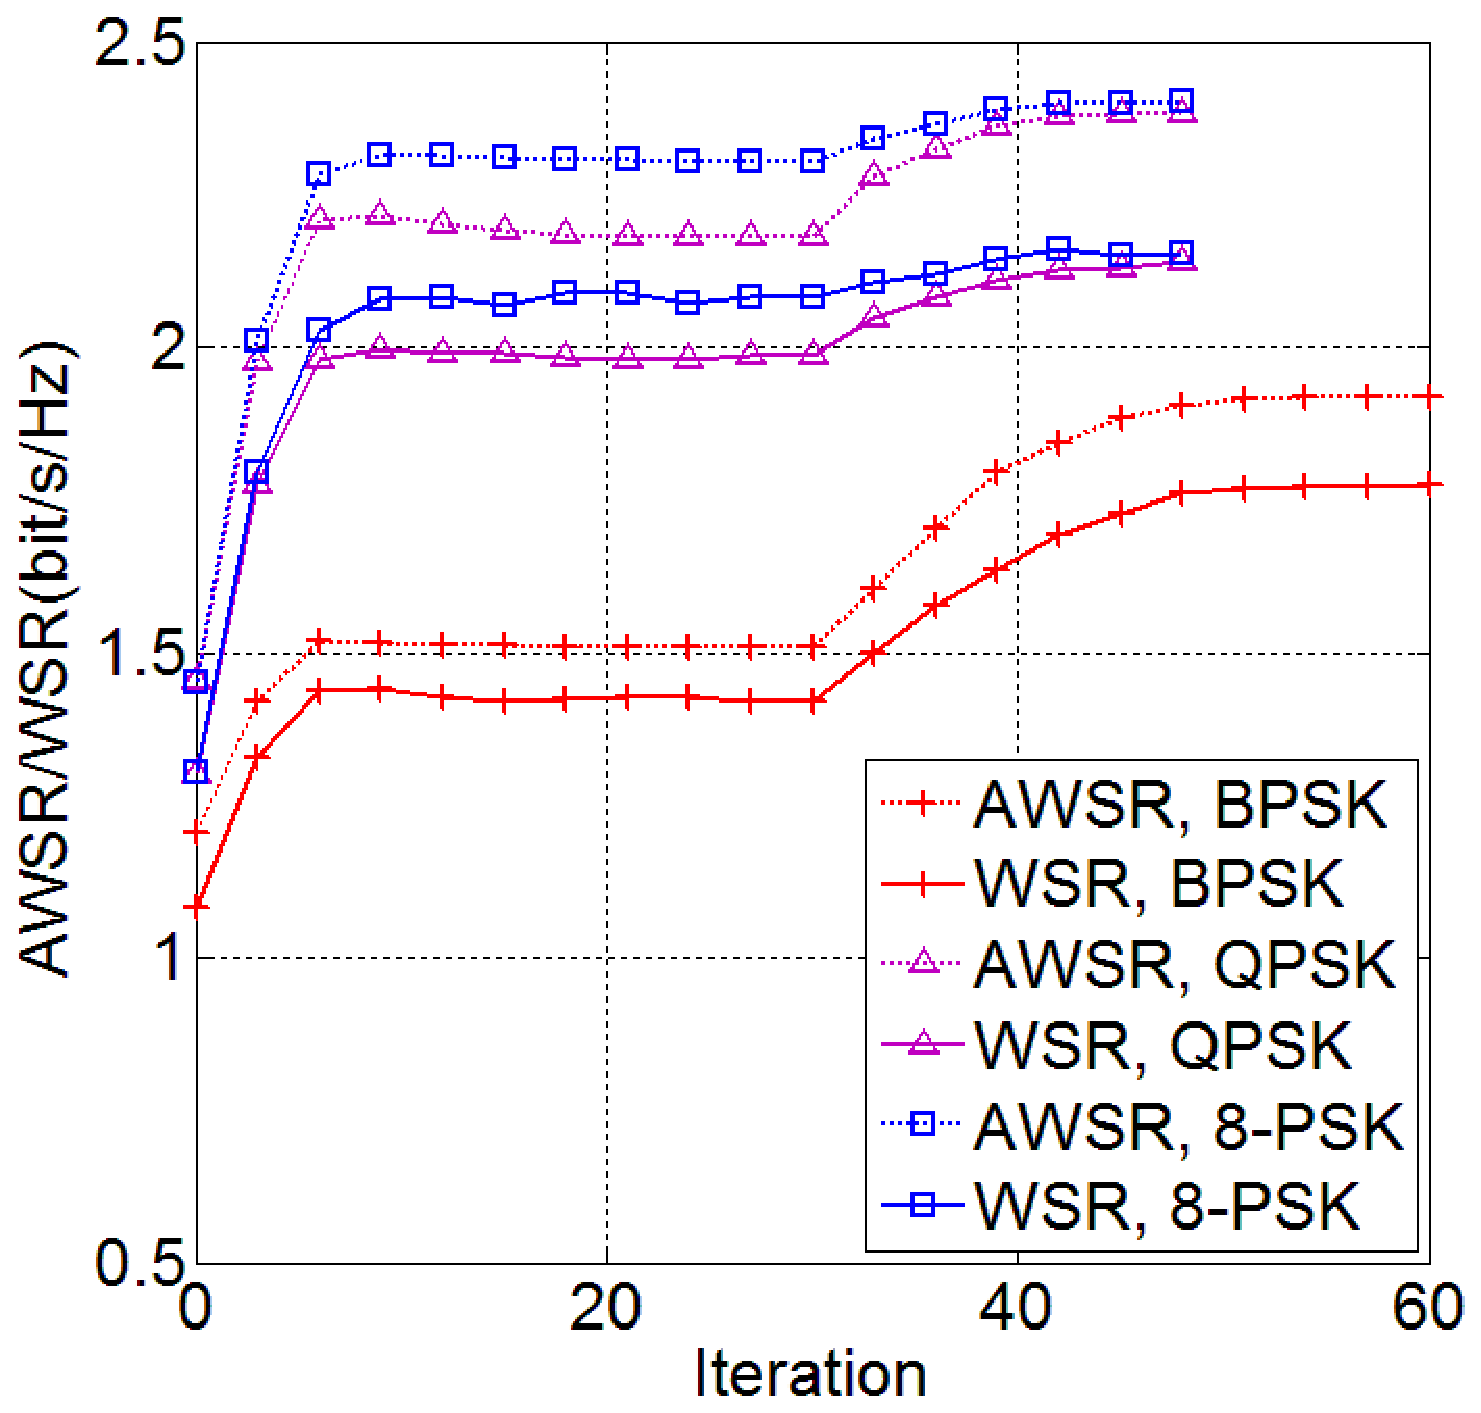
\includegraphics[width=4.0cm]{RecordGP1SGDPConvergence.eps}}
          \centerline{(a) GP1 + S-GDP}\medskip
        \end{minipage}
        \hfill
        \begin{minipage}[b]{.48\linewidth}
          \centering
          \centerline{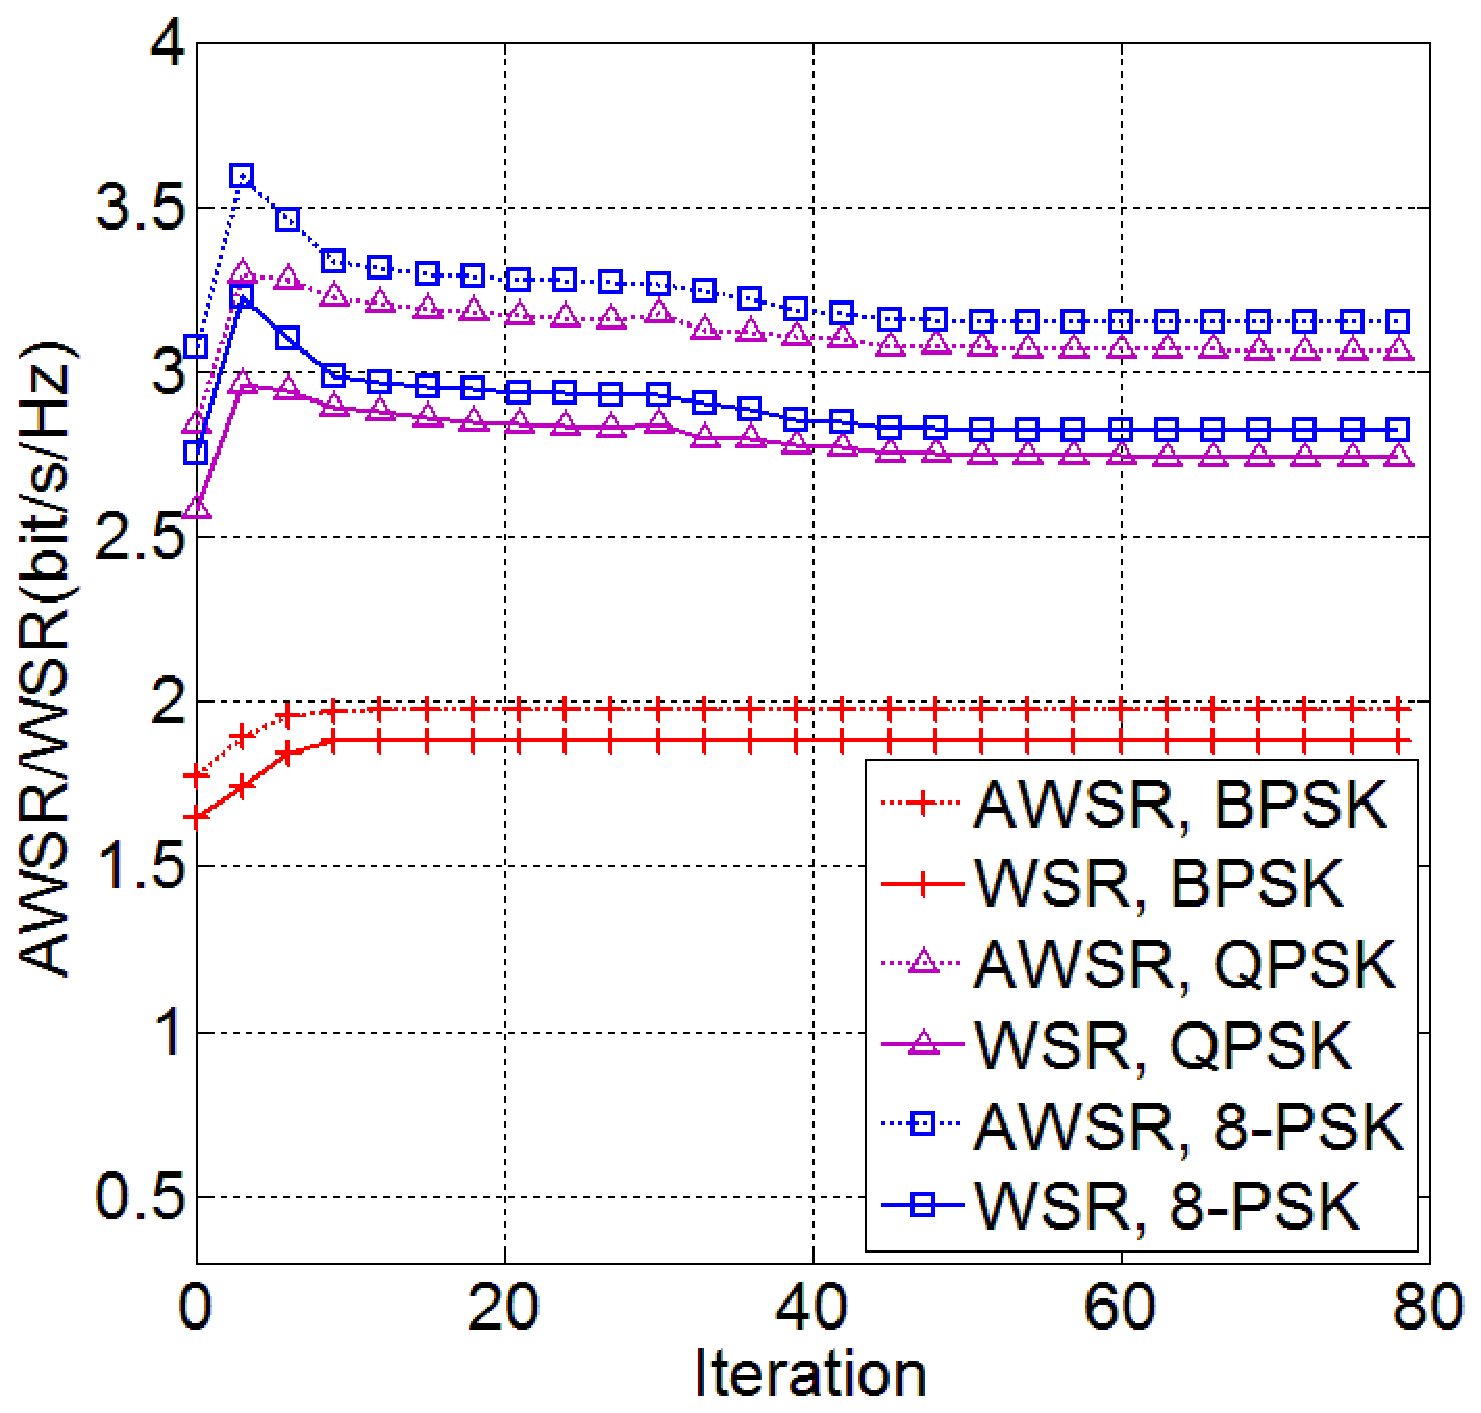
\includegraphics[width=4.0cm]{RecordBDAGDPConvergence.eps}}
          \centerline{(b) B-GDP}\medskip
        \end{minipage}

        \caption{Convergence behavior of (a) GP1 + S-GDP and (b) B-GDP}
        \label{fig:Convergence}
    \end{figure}

    \begin{figure}[!h]
        \centering
        \centerline{\includegraphics[width=\columnwidth]{RecordGP1SGDP_GP1.eps}}
        \vspace*{-3mm}
        \caption{Comparison between GP1 + S-GDP and GP1.}
        \label{fig:GP1SGDP_GP1}
    \end{figure}


    \begin{figure}[!h]
        \centering
        \centerline{\includegraphics[width=\columnwidth]{RecordBDAGDP_GP2.eps}}
        \vspace*{-3mm}
        \caption{Comparison between B-GDP and GP2.}
        \label{fig:BDAGDP_GP2}
    \end{figure}
}

\vspace*{-3mm}

\section{Conclusion}
\label{sec:con}
\vspace*{-2mm}

This work investigates the design optimization of linear precoders in multi-cell MIMO downlink channel (MC-MIMO-DLC)
with known finite-alphabet inputs.  In our approach,
we first simplify the complexity to evaluate the finite-alphabet weighted sum rate (WSR) and its gradient by adopting an approximation
to Monte-Carlo sampling and derive a simple gradient descent algorithm (S-GDP) for precoder optimization. Second,
by enforcing block diagonalization restriction whenever possible, we derive an alternating gradient
descent precoder optimization algorithm (B-GDP) based on
two convex subproblems: One uses Stiefel manifold method and the other utilizes dual decomposition.
Our numerical tests demonstrate the superior
convergence behaviors and the performance advantages of
both S-GDP and B-DGP algorithms over existing methods given finite-alphabet inputs.

\vfill\pagebreak
% References should be produced using the bibtex program from suitable
% BiBTeX files (here: strings, refs, manuals). The IEEEbib.bst bibliography
% style file from IEEE produces unsorted bibliography list.
% -------------------------------------------------------------------------

\bibliographystyle{IEEEbib}
\bibliography{myrefs}

\end{document}

